%!TEX root = ../thesis.tex
%Adding the above line, with the name of your base .tex file (in this case "thesis.tex") will allow you to compile the whole thesis even when working inside one of the chapter tex files

\chapter{Radio Interferometric Data Analysis} \label{chap:4}

The complex visibilities outputted from the correlator of a radio interferometer are far from ideal and many additional steps of processing are required before they can be of scientific use. The imperfection of the synthesis radio telescopes (e.g., surface accuracy, receiver noise, gain stability, etc.), the adjustments to the signal (e.g., filter bandpass, etc.), hardware or software failures, poor atmospheric conditions, and the presence of RFI are some of the many sources of visibility corruption that must be accounted for before they can be Fourier transformed to get the sky brightness distribution. The chapter describes the three main steps involved in reducing any standard radio interferometric data set, namely: data examination and flagging, data calibration, and imaging. In each step we give relevant examples of the data reduction techniques used in \cite{ogorman_2012} and \cite{ogorman_2013}. A general work flow chart is given in Figure \ref{fig:4.1} which highlights the standard procedure required to go from raw visibilities to image analysis and summarizes what will be discussed in this chapter.\\
\\
\begin{figure}[hbt!]
\centering 
          \includegraphics[trim=20pt 220pt 0pt 200pt,clip,scale=0.74]{/home/eamon/thesis/thesis_template/4/cash_flow.ps}
\caption[Radio interferometry work flow chart]{Work flow chart highlighting the general procedure required to go from the raw visibilities outputted by the correlator to a final radio image that can be used for scientific analysis. (Image adapted from the CASA cookbook, NRAO)}
\label{fig:4.1}
\end{figure}

\section{Data Examination and Flagging}\label{sec:4.1}
The Common Astronomy Software Application \citep[CASA;][]{mcmullin_2007} package was used to flag, calibrate, and image the main data sets used in this thesis. CASA is operated through a Python interface and uses a suite of astronomical data reduction tools which have been developed to meet the processing requirements of the large  data sets from the Karl G. Jansky VLA and ALMA. It can also be used to process data from practically all other modern radio synthesis arrays. For synthesis data to be processed in CASA, it must be in a ``measurement set'' format. VLA data is easily transferable into this format using the \textit{importevla} task within CASA. CARMA data files however come in \textit{Miriad} format and need to be first converted into Flexible Image Transport System (FITS) format within the Miriad \citep{sault_1995} data reduction package. During this process the raw data are smoothed by a Hanning filter (combining adjacent frequency channels with weights 0.25, 0.5, and 0.25) to dampen ringing in the bandpass. Once in FITS format, the data can then be imported into CASA using the \textit{importuvfits} task.

Once the data has successfully been imported into CASA the \textit{listobs} task can be used to get a summary of the data set, allowing the user to make sure the observing track contains the requested sources observed at the correct times. At this point it is also a good idea to check any observing logs which are created on site during the observation by the array operators. These logs contain important information about specific tracks such as non-operational antennas or unavailable receivers, and such data will either need to be treated appropriately during calibration or flagged at this stage. The \textit{plotms} task, which is a GUI-style plotter, can then be used to obtain X-Y plots of the visibility data. A good visual overview of the observation track is obtained by plotting all the source visibility amplitudes as a function of time. Averaging the data over channels or baselines often alerts the user to obvious bad data, which can be manually flagged through the \textit{plotms} interface or through the \textit{flagdata} task. An example of such a plot is shown in Figure \ref{fig:4.2} where the visibility amplitudes of three sources in a 1.3\,cm VLA observing track for Aldebaran are displayed against time. The relatively weak target is shown between interleaving scans of the stronger phase calibrator, while the flux calibrator is the scan at the end of the observing track and is the strongest source in this observation. The data can be averaged over channels or baselines to speed up the plotting process. Some relatively low visibility amplitudes can clearly be seen for all scans of the phase calibrator, which can be traced to a single poor performing antenna.

\begin{figure}[hbt!]
\centering 
\includegraphics[trim=20pt 240pt 0pt 230pt,clip,scale=0.75]{/home/eamon/thesis/thesis_template/4/c_overview.ps}  
\caption[Examination of a VLA data set]{Data examination of a 6\,cm VLA data set for Aldebaran. A good visual overview of the observation track is obtained by plotting all the source visibility amplitudes as a function of time. Averaging the data over channels or baselines sometimes allow rogue data to stand out. Here the black, orange, and green data points represent the phase calibrator, the science source, and the flux calibrator, respectively. The left most black data points are part of the dummy scan which was subsequently flagged. The low data points of the phase calibrator are data which needs further investigation. The absence of data at certain times represent observations at 3\,cm.}
\label{fig:4.2}
\end{figure}

Another important way to represent the data at this stage of the flagging process is to plot the visibility amplitude of each of the sources as a function of $u-v$ distance or baseline length (i.e., $\sqrt{u^2 + v^2}$). The amplitude distribution should be relatively constant as a function of $u-v$ distance for the phase calibrator (i.e., a point source) and will fall off with increasing baseline length if the flux calibrator is resolved. Plotting the data in this format often results in extreme points at certain baselines which can then often be traced back to poorly behaving antennas or corrupt baselines. There is also some flagging which can be carried out based in part on a priori information. Antennas in very compact configurations can partially block the incoming RF signal to other antennas, which is often referred to as antenna shadowing. This was not a problem in our VLA B configuration observations but some data obtained in the more compact CARMA configurations had to be flagged as a result of this shadowing. At the time when our VLA observations took place, every observing track (i.e., scheduling block) needed to commence with at least a one minute \textit{dummy scan} to facilitate the correlator setup. We subsequently flagged these scans as they contained no useful scientific data. Other a priori flagging was to remove any visibilities with zero amplitudes and to flag the edge channels in the CARMA data sets. Finally, visual inspection of each scan was carried out to determine if data at the beginning or end of these scans needed to be flagged. This process is often referred to as quacking in radio interferometry analysis.

No RFI was present in any of the CARMA data sets and in any of the VLA data sets at wavelengths $\lesssim 3$\,cm (i.e., X, K, Ka, and Q bands). For the 2011 long wavelength ($> 3$\,cm) data, the two sub-bands were centered at relatively RFI free regions of the bandpass and only a very small amount of RFI had to be manually flagged. The 2012 wide-band data were taken at 10 and 20\,cm (i.e., S and L band) and many of the sub-bands were severely contaminated with RFI, especially at 20\,cm. In Figure \ref{fig:4.3} we plot the visibility amplitude of the flux calibrator 3C286 against frequency for the 2012 wide-band data set at 20\,cm. The upper panel shows the raw data before any RFI had been removed. Some of the sub-bands were badly contaminated with RFI ($>90\%$) and had to be completely flagged. The remaining sub-bands were initially Hanning smoothed to suppress Gibbs ringing. This action spreads the single-channel RFI into three channels, but importantly removes the effects of some of the worst RFI from a number of channels and allows as much good data to be retained as possible. The \textit{testautoflag} task was then used to conservatively flag RFI from all sources and any remaining RFI was manually flagged. The final result for the flux calibrator is shown in the bottom panel of Figure \ref{fig:4.3} with only some residual RFI still remaining, particularly between 1 and 1.2\,GHz.

\begin{figure}[hbt!]
\vspace{9mm}
\centering 
\includegraphics[trim=30pt 70pt 20pt 70pt,clip,width=14cm,height=16cm]{/home/eamon/thesis/thesis_template/4/rfi_thesis_new.ps}  
\caption[Eliminating RFI from the L band data set]{Eliminating RFI from the 20\,cm wide-band data set. \textit{Top panel:} Raw visibility amplitudes showing the presence of high levels of RFI in many sub-bands. \textit{Bottom panel:} Post flagging visibility amplitudes. Some of the sub-bands were so severely contaminated with RFI that they had to be completely flagged. The data is still uncalibrated at this stage and the gain as a function of frequency is clearly present.}
\label{fig:4.3}
\end{figure}

\section{Calibration}\label{sec:4.2}

The role of calibration is to correct the measured visibilities $V'(u,v)$ to approximate as closely as possible the true visibilities $V(u,v)$. As discussed in Chapter \ref{chap:2}, the true visibilities are related to the sky brightness via the Fourier transform:
\begin{equation}
V_{ij}[u_{ij}(t),v_{ij}(t)] = \int A(l,m) I(l,m) \mathrm{exp}[-i2\pi(u_{ij}(t)l + v_{ij}(t)m)]	dl	dm
\end{equation}
where $i,j$ represent the discrete sampling of the antennas $i$ and $j$, at time $t$. The term $u_{ij}(t)l + v_{ij}(t)m$ is the geometric phase difference produced by the geometric path length difference between antenna $i$ and antenna $j$ from the source (or part of) at location ($l,m$) relative to the phase center. The relationship between the measured visibility and the true visibility on a baseline between antennas $i$ and $j$ may be expressed as
\begin{equation}
V_{ij}' =  J_{ij}V_{ij}
\end{equation}
where $ J_{ij}$ represents the accumulation of all corruptions affecting baseline $ij$. This equation is known as the Hamaker-Bregman-Sault Measurement Equation \citep{hamaker_1996}. The most important of the effects contained in $J_{ij}$ are antenna-based and arise from the measurable physical properties of individual antenna elements or the measurable physical conditions in the atmosphere above them. Thus, an array of $N$ antennas forming $N(N-1)/2$ baselines can usually be adequately calibrated through the determination of only $N$ factors.

For the purpose of the work presented in this thesis, the Measurement Equation can be written as
\begin{equation}
V_{ij}'(u,v,\nu) = b_{ij}(t)[B_{i}(\nu ,t)B_{j}^{*}(\nu ,t)]g_{i}(t)g_{j}(t)V_{ij}(u,v,\nu)e^{i[\theta _{i}(t) - \theta _{j}(t)]}
\end{equation}
where
\begin{itemize}
\item $g_{i}$ and $\theta _{i}$ are the amplitude and phase portions of the complex gain. These are usually determined separately in the calibration process and may change over the observation period due to factors such as temperature, atmospheric conditions, etc. 
\item $B_{i}$ is the complex bandpass, the instrumental response as a function of frequency, $\nu$, and may also vary over time.
\item $b_{ij}(t)$ is the baseline term and is important shortly after a configuration change when antenna positions may not be well known.
\end{itemize}
The general calibration strategy is then to derive a series of scaling factors from both the phase and flux calibrators, which are then collectively applied to the science target in the final stage of calibration. A general workflow diagram describing the main steps involved in calibration process are summarized in Figure \ref{fig:4.4}. We now discuss each of these steps while placing emphases on our CARMA and VLA data.

\begin{figure}[t!]
\centering 
\includegraphics[trim=20pt 160pt 0pt 140pt,clip,scale=0.6]{/home/eamon/thesis/thesis_template/4/calib_overview.ps}  
\caption[Calibration workflow diagram]{A workflow diagram outlining the main steps involved in calibrating radio interferometric data. Each of these steps are discussed in the text in relation to our CARMA and VLA observations (CASA cookbook, NRAO).}
\label{fig:4.4}
\end{figure}

\subsection{Prior Calibration}
Our 2011 VLA data were acquired just after an array re-configuration, which meant that the positions of some of the antennas were not accurately known at the time of observations. This resulted in some data points having inaccurate $u-v$ coordinates. During the course of observations in each configuration, the exact position of all antennas become known and so the $u-v$ data could be calibrated to account for the discrepancies in the $u-v$ coordinates.  At the VLA site, atmospheric opacities become significant at frequencies $\gtrsim 20$\,GHz as shown in Figure \ref{fig:4.5} and so opacity corrections were applied to the high frequency data sets. The adjustment values were based on the average of a seasonal model (based on many years of measurements) and information from the weather station obtained during the observations. For the CARMA data, the opacity at 1.3\,mm is measured by a tipper \citep{white_2009}. The tipper reflects radiation from the blank sky at different inclinations onto a radiometer. The voltage from the radiometer can then be plotted against inclination to allow the opacity to be calculated. 

\begin{figure}[t!]
\centering 
\includegraphics[trim=20pt 320pt 0pt 300pt,clip,scale=0.7]{/home/eamon/thesis/thesis_template/4/opacity.ps}  
\caption[Atmospheric opacity at the VLA site]{Calculation of the atmospheric opacity at the VLA site between $1-50$\,GHz on 2011 February 11. The adjustment values applied to the data were based on the average of a seasonal model and information from the weather station obtained during the observations.}
\label{fig:4.5}
\end{figure}

The final a priori calibration step is to provide a flux density value to the flux calibrator via CASA's \textit{setjy} task. The VLA flux calibrators were assigned values using the ``Perley-Butler 2010" flux density standard models  and with assumed systematic uncertainties of 3\% at all frequencies \citep{perley_2013}. At the time, no Ka or S band flux density standard models were available so instead for these we used the K and L band models, respectively, which were scaled according to their spectral indices. The absolute flux scale for CARMA observations is often determined by observing a planet and using a model of its flux as a function of baseline length. However, no such models were available in the earlier versions of CASA which we used at the time and so the flux calibration was carried out with the quasers, 0530+135 and 3C120. The continuously updated CARMA flux catalog was accessed via the \textit{xplore} GUI to obtain their flux values at each observation. The flux of these objects are more unpredictable and the systematic uncertainties are about 20\%.

\subsection{Bandpass Calibration}
The bandpass is the relative gain as a function of frequency and solving for it is the first part of the calibration process. Variation in frequency arises from frequency dependent effects in signal transmission. Such variation is shown in Figure \ref{fig:4.6} for both phase and amplitude for a single antenna. For the VLA data, the flux calibrators were also used as the bandpass calibrators. Their phases were found to vary significantly over the $5-10$ minutes of observation especially at high frequencies; in most cases by a few 10s of degrees. Before a solution to the bandpass could be found, these phase variations needed to be corrected, to prevent decorrelation of the vector averaged bandpass solution. The complex bandpass, $B_i$, could then be solved using the \textit{bandpass} task and applying the antenna positions and phase solutions. The bandpass solutions  were then applied to the bandpass calibrator to check that both the amplitude and phase were then almost constant across channels/frequency.

The CARMA data contained three spectral windows (i.e., 468, 62, and 31\,MHz in width), each having independent bandpass shapes in both amplitude and phase. In theory, one could calculate the bandpass of each spectral window individually by observing a bright astronomical source. However, for narrow spectral windows this would be too costly in observing time in order to reach a sufficient S/N. Thankfully, for each of these spectral windows, the gain calibrations are typically the same  after the full bandpass dependence has been removed. The strategy to calibrate the CARMA data was to initially carry out the bandpass calibration on the wideband data (i.e., 468\,MHz) using the same strategy outlined in the previous paragraph, and then carry out the gain calibration on this wideband data. Once this had been done, these bandpass independent gain solutions were applied to the narrow band data (i.e., 62, and 31\,MHz) while solving for their bandpass. This narrow band bandpass solution could then be applied to the target and phase calibrator.

\begin{figure}[t!]
\centering 
\includegraphics[trim=20pt 320pt 0pt 300pt,clip,scale=0.77]{/home/eamon/thesis/thesis_template/4/bandpass.ps}  
\caption[Gain variation as a function of frequency]{One antenna's gain variation as a function of frequency for the flux calibrator 3C138 at 1.3\,cm. Bandpass calibration corrects for this variation.}
\label{fig:4.6}
\end{figure}

\subsection{Gain Calibration}

Once a bandpass solution has been applied, the next step is to derive corrections for the antenna amplitude and phase gains, $g_{i}$ and $\theta _{i}$, as a function of time. The amplitude changes on a much longer timescale than the phase and so they are solved separately. The general procedure then is to solve for these antenna-based gain factors for each scan on all calibrators. In order to determine the appropriate antenna-based complex gains for the science target, a phase calibrator which is always a point source and located much closer to the target than the flux calibrator, is regularly observed to minimize differences through the atmosphere. If there is a substantial change in phase over a scan, and the uncorrected phases were averaged over this timescale, then the amplitude would be decorrelated. It is therefore important to correctly determine appropriate scan lengths when preparing the observations, especially at high frequencies, where  time-dependent gain errors are introduced by the troposphere.

During gain calibration, the relative gain amplitudes and phases for different antennas are determined using the phase calibrator. The \textit{gaincal} task is used to do this. The absolute flux density scale of the phase calibrator is later determined by comparison against the gain amplitudes $g_{i}$ derived for the flux calibrator. To find the relative phases, a zero phase is determined by selecting a reference antenna for which the phase is defined to be zero. In the first step new solutions of complex gains $g_{i}$ and $\theta _{i}$ are derived for the flux density calibrator which are corrected for the bandpass shape (here we assume the flux density calibrator has been used as the bandpass calibrator as was the case for our observations). The second and final step requires the determination of the appropriate complex gains from the phase calibrator.

\subsection{Flux Scale Calibration and Application of Solutions}\label{subsec:2.4}
The penultimate stage of the calibration process is to use the known flux density of our flux calibrator (whose flux density was set using \textit{setjy}) to derive the flux density of the phase calibrator, which was previously assumed to be a point source of 1\,Jy located at the phase center. This is achieved using the \textit{fluxscale} task. The final step of the calibration process is to apply the calibration solutions to all the targets, using the task \textit{applycal}. During this process, the calibration solutions are applied to the DATA column in the measurement set, and the results are written in the CORRECTED$\_$DATA column of the measurement set. For the calibrators, the phase and amplitude calibration solutions comes from their own solutions and the bandpass solutions come from the bandpass calibrator. For the science target we again apply the bandpass solution of the bandpass calibrator but the gain solutions come from the nearby phase calibrator.

\begin{figure}[hbt!]
\centering 
\includegraphics[trim=20pt 240pt 0pt 220pt,clip,scale=0.77]{/home/eamon/thesis/thesis_template/4/calib_x_phase_amp.ps}  
\caption[Example of a well calibrated source]{A well calibrated source will produce a compact ball of visibilities centered at zero phase and at the amplitude found for that source. Here we plot the calibrated visibilities at 3\,cm for J0449+1121; the phase calibrator in the 3\,cm data set for Aldebaran.}
\label{fig:4.7}
\end{figure}

Once calibration of the data is complete, it is worth spending time inspecting the corrected data to make sure there are no obvious errors in the data. If such errors are indeed found at this stage, then their cause will need to be flagged and the data must be re-calibrated. Some insightful plots to investigate how successful the calibration was, are: amplitude vs. time, amplitude vs. $u-v$ distance, and amplitude vs. phase. If a point source has being successfully calibrated then it will have an appearance similar to that in Figure \ref{fig:4.7}, i.e., a compact ball of visibilities centered at zero phase and at the amplitude found for that source. Once the data has been successfully calibrated, the science data is split off into a separate measurement set using the \textit{split} task. The calibrated visibilities can then be either directly analyzed by fitting simple models (e.g., point sources, disks, etc.,) to them or, as is more common, Fourier transformed and CLEANed to create an image of the source.

\section{Imaging}\label{sec:4.3}
We have shown in Chapter \ref{chap:2} that the visibility as a function of baseline coordinates $(u,v)$ is the Fourier transform of the sky brightness distribution as a function of the sky coordinates $(l,m)$, i.e.,
\begin{equation}
I(l,m)=\int \int V(u,v)e^{2\pi i(ul +vm)}dudv.
\end{equation}
Taking the inverse Fourier transform of the calibrated visibilities results in a dirty image which can then be deconvolved to produce a good estimate of the true sky brightness distribution. CASA has a single task called \textit{clean} which carries out both of these operations on the data. In the following two sections we describe how both the VLA and the CARMA visibility data sets were imaged using this task.

\subsection{Imaging the VLA Data}\label{sec:4.3.1}

The calibrated visibilities were both inverse Fourier transformed and deconvolved using the CASA \textit{clean} task in multi-frequency synthesis imaging mode. This imaging mode separately grids the multiple spectral channels onto the \textit{u-v} plane and therefore improves the overall \textit{u-v} coverage. As all science targets were expected to be point sources at all wavelengths, resolution was not paramount and so we used natural weighting for maximum sensitivity. The cell size was chosen so that the synthesized beam was about five pixels across. The FOV of the VLA at short wavelengths is small (see Table \ref{tab:3.6}) and at these wavelengths there are less serendipitous background objects. This meant that the science targets were the only objects within a few primary beams of the phase center and so it was sufficient to place just one CLEAN circle around the target source. The general procedure was to first use \textit{clean} to create a dirty image (i.e., by setting \textit{niter}\,=\,0) allowing the root mean square noise of this dirty image, $\sigma _{\rm{rms}}$, to be determined. The final CLEAN image was then created by setting \textit{niter} to a very large number  and setting the CLEANing threshold to be $\sim 3\sigma _{\rm{rms}}$. Setting \textit{niter} to a very large number ensures that this CLEANing threshold is reached.

\begin{figure}[t!]
\centering 
\vspace{28mm}
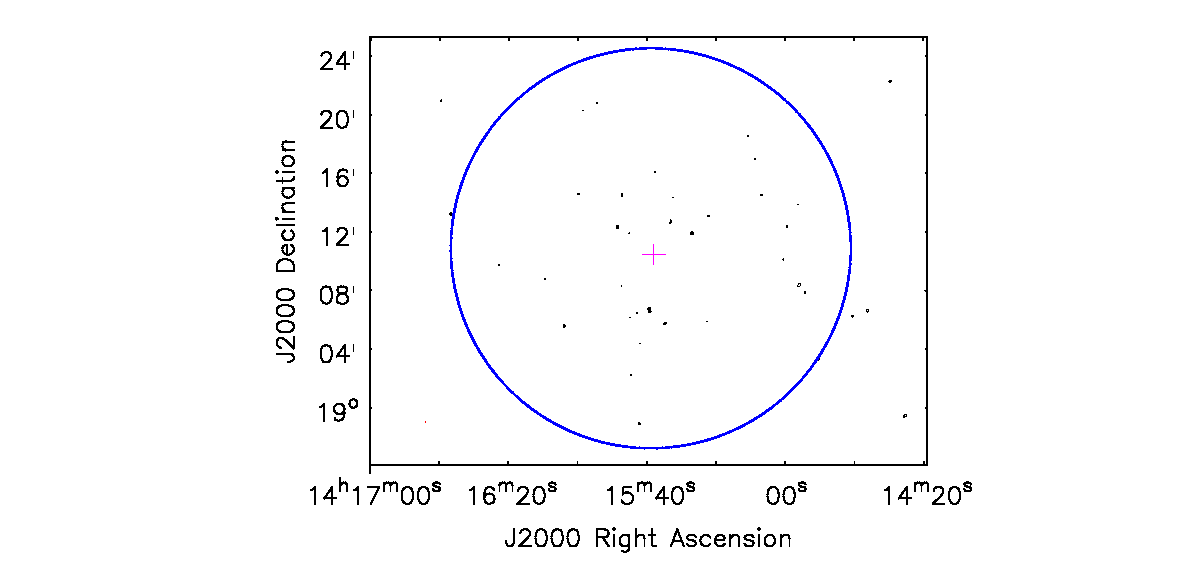
\includegraphics[trim=130pt 0pt 100pt 0pt,clip,width=15cm,height=12.5cm]{/home/eamon/thesis/thesis_template/4/l_thesis.ps}  
\caption[Wide field view of the VLA 20\,cm image]{Wide field view of the VLA 20\,cm CLEANed image showing the many serendipitous background sources close to Arcturus (pink cross). Many of these sources were a few orders of magnitude brighter than Arcturus at 20\,cm. CLEAN circles were placed around all these sources during interactive CLEANing. The blue circle marks the FOV (i.e., the HPBW of the primary beam) of the VLA at 20\,cm while the pink cross in the center marks the position of Arcturus. The contour levels are set at $(0.005,0.01,0.05,0.1,0.2,0.4,0.6,0.8)\times 80.3$\,mJy, where $80.3$\,mJy is the flux of the brightest source in the image.}
\label{fig:4.8}
\end{figure}

At long VLA wavelengths the primary beam becomes larger and the background sky sources become brighter. The new wide bandwidth capabilities of the VLA means that it is quite sensitive to emission far from phase center. For example, at $\sim 20$\,cm (L band), the HPBW of the primary beam is $\sim 30^{\prime}$ and yet the primary beam gain is as much as 10\% around $1^{\circ}$ away. In Figure \ref{fig:4.8} we show a wide field view of our VLA 20\,cm image clearly showing many serendipitous sources out to and beyond the HPBW of the primary beam, all of which needed to be individually CLEANed to reduce their sidelobe contamination of the final image. For this reason the image sizes were usually set to a few times the size of the primary beam (if not too computationally expensive) so that any nearby strong serendipitous sources could be CLEANed. These images were again CLEANed interactively while taking sky curvature into account. CLEANing was carried out interactively with CLEAN circles first placed around the strongest sources in the image and then placing them around weaker sources as they appeared in the residual image. 
 
\subsection{Imaging the CARMA Data}\label{sec:4.3.2}

The CO emission around Betelgeuse is extended and has many different spatial scales. Traditional deconvolution techniques such as the CLEAN and MEM algorithms are scale-free and have no concept of source size. Both algorithms treat each pixel as an independent degree of freedom. However, adjacent pixels in an image are not independent due to the limiting resolution set by the dirty beam and the intrinsic source size. For example a Gaussian source covering 50 pixels can be characterized by only 5 parameters, not 50. The CASA multi-scale algorithm uses ``Multi-scale CLEAN'' \citep{cornwell_2008} which is a scale sensitive algorithm that employs fewer degrees of freedom to model plausible sky brightness distributions. Instead of deconvolving using just delta-functions (or pixels) as in other clean algorithms, Multi-scale CLEAN carries out the deconvolution using delta-functions and circular Gaussians of various scales. It has been shown to produce more realistic representations of the sky brightness distribution for extended complex emission than the traditional CLEAN algorithm does \citep{rich_2008}.

\begin{figure}[hbt!]
\vspace{10mm}
\centering 
\mbox{
\includegraphics[trim=127pt 0pt 130pt 0pt,clip,scale=0.7]{/home/eamon/thesis/thesis_template/4/thesis_clean.eps}  
\includegraphics[trim=127pt 0pt 130pt 0pt,clip,scale=0.7]{/home/eamon/thesis/thesis_template/4/thesis_multi.eps}  
}
\mbox{
\includegraphics[trim=127pt 0pt 130pt 0pt,clip,scale=0.7]{/home/eamon/thesis/thesis_template/4/thesis_clean_resid.eps}  
\includegraphics[trim=127pt 0pt 130pt 0pt,clip,scale=0.7]{/home/eamon/thesis/thesis_template/4/thesis_multi_resid.eps}  
}
\caption[Comparing CLEAN to Multi-scale CLEAN]{Comparing CLEAN to Multi-scale CLEAN using one of the combined configuration CARMA channel maps at -14.1\,km\,s$^{-1}$. The top panel shows the final deconvolved images using CLEAN (left) and Multi-scale CLEAN (right) with the emission in both maps truncated between 0 and 0.2\,Jy\,beam$^{-1}$ to enhance weak emission. Multi-scale CLEAN is more successful at recovering large-scale structure. The bottom panel shows the residual images after using CLEAN (left) and Multi-scale CLEAN (right) where the emission in both images have been truncated between 0 and 0.06\,Jy\,beam$^{-1}$. The emission appears more noise-like in the Multi-scale residual image while the CLEAN residual image contains some uncleaned flux.}
\label{fig:4.9}
\end{figure}

Multi-Scale CLEAN is really just a modification of the classical CLEAN algorithm. It assumes that sources in the sky are actually extended structures of different scales (which can include point sources), unlike the traditional CLEAN algorithm which assumes the sky is empty apart from a limited number of point sources. The function used to define the shape of the different spatial scales (usually a truncated circular Gaussian) has a finite extent and becomes a delta-function in the limit of zero scale-size. The Multi-scale CLEANing process is then as follows:
\begin{enumerate}
\item The dirty map is convolved with each scale size to create $n$ convolved images, where $n$ is the number of defined scale sizes.
\item The global scale among these images that contains the maximum total flux has its position, flux, and scale size recorded.
\item The pre-computed scale in which the peak was found, is convolved by the dirty beam, multiplied by some gain factor, and the subtracted from all the images made in the first step.
\item The subtracted component and its scale size is stored in a table.
\item Steps $1-4$ are repeated until a flux threshold is reached in one of the residual images.
\end{enumerate}
The new model is then convolved with a CLEAN beam and the residuals are added to it to get the restored image.

The combined CARMA configuration image cubes were Multi-scale CLEANed down to the 3$\sigma _{\rm{rms}}$ threshold. Natural weighting was applied to the $u-v$ data to optimize the sensitivity for the weak CO emission and the CLEAN region was set to be about the size of the HPBW of the primary beam. The Multi-scale algorithm  within CASA was set to four unique scales; the largest corresponding to the largest structures visible in individual channel maps. Each scale was approximately set to three times smaller than the preceding scale and a zero-scale was included to account for point sources. In Figure \ref{fig:4.9} we plot one channel from the final restored image cube and compare this to the same channel from an image cube that was deconvolved using the traditional CLEAN algorithm. It can clearly be seen that Multi-scale CLEAN produces more extended emission around the star. This is because Multi-scale CLEAN removes large-scale structure before finer details while the CLEAN algorithm cannot distinguish noise peaks from faint real signals \citep{rich_2008}. We also include the resultant residual images from both algorithms in the bottom panel of Figure \ref{fig:4.9}. The CLEAN residual image still contains some uncleaned flux while the emission appears more noise-like in the Multi-scale residual image.